\documentclass[conference]{IEEEtran}
\IEEEoverridecommandlockouts
\usepackage{cite}
\usepackage{amsmath,amssymb,amsfonts}
\usepackage{graphicx}
\usepackage{url}
\usepackage{textcomp}
\usepackage{xcolor}
\usepackage{booktabs}
\usepackage{multirow}
\usepackage{array}
\usepackage{tikz}
\usepackage{algorithm}
\usepackage{algorithmic}
\usepackage{enumitem}
\usepackage{subcaption}
\usetikzlibrary{shapes.geometric, arrows.meta, positioning, calc}

\def\BibTeX{{\rm B\kern-.05em{\sc i\kern-.025em b}\kern-.08em
    T\kern-.1667em\lower.7ex\hbox{E}\kern-.125emX}}

\makeatletter
\newcommand{\linebreakand}{%
  \end{@IEEEauthorhalign}
  \hfill\mbox{}\par
  \mbox{}\hfill\begin{@IEEEauthorhalign}
}
\makeatother

\tikzset{
  pbox/.style={
    rectangle, rounded corners=4pt,
    draw=black!70, fill=white,
    text width=7.6cm, align=center,
    minimum height=0.85cm, font=\scriptsize\sffamily, inner sep=4pt
  },
  arr/.style={
    -{Stealth[length=4pt,width=3pt]},
    black!60, line width=0.55pt
  },
}

\begin{document}

\title{Calibrating Conservatism in Offline Reinforcement Learning\thanks{Code, data, and reproduction instructions: \url{https://github.com/enigmatronix13/Calibrating-Conservatism-in-Offline-Reinforcement-Learning}.}}

\author{%
\IEEEauthorblockN{Kaaviya Kalyanakumar\IEEEauthorrefmark{1}}
\IEEEauthorblockA{\textit{Manipal Institute of Technology}, Manipal, India\\
  kaaviya.mitmpl2023@learner.manipal.edu}
\and
\IEEEauthorblockN{Kashvi Ranjan\IEEEauthorrefmark{1}}
\IEEEauthorblockA{\textit{Manipal Institute of Technology}, Manipal, India\\
  kashvi1.mitmpl2023@learner.manipal.edu}
\linebreakand
\IEEEauthorblockN{Dr.\ G.\ Pradeep Reddy}
\IEEEauthorblockA{\textit{Manipal Institute of Technology}, Manipal, India\\
  pradeep.reddy@manipal.edu}
\and
\IEEEauthorblockN{Dr.\ Upadrasta Shivani Sri Varshini}
\IEEEauthorblockA{\textit{Manipal Institute of Technology}, Manipal, India\\
  shivani.srivarshini@manipal.edu}
\thanks{\IEEEauthorrefmark{1}These authors contributed equally to this work.}
}
\maketitle

\begin{abstract}
Conservative Q-Learning applies a fixed, globally uniform penalty to value
estimates regardless of local data coverage. We test whether that penalty is
spatially miscalibrated across three D4RL datasets spanning two domains:
path-concentrated navigation (\texttt{maze2d-medium-sparse-v1},
\texttt{maze2d-large-sparse-v1}) and dense-reward locomotion
(\texttt{hopper-medium-v2}). Seven offline RL methods (TD3-BC, CQL,
Q-ensemble, BEAR, UWAC, MOPO, APTQ-CQL) are trained under a matched
PyTorch protocol with Bellman backups, target critics, per-domain reward
scaling, and three random seeds, then ranked by a unified offline
policy-value proxy (mean $Q(s,\pi(s))$ on held-out dataset states) and
analysed with coverage-tier Conservative Excess Ratio (CER) and
Uncertainty--Return Correlation (URC) diagnostics. The proxy ranking is
\emph{stable across all three datasets}: CQL highest, APTQ-CQL second, with
the remaining baselines an order of magnitude lower. Coverage-tier CER shows
both CQL and APTQ-CQL are optimistic relative to a Monte Carlo value
baseline ($\mathrm{CER}{<}0$) in every tier and dataset, and APTQ-CQL
consistently reduces this excess---most strongly in well-covered tiers.
Critically, URC \emph{flips sign by domain}: positive on the sparse mazes
(uncertainty fails to track return risk) but negative on hopper
(uncertainty anticorrelates with return), showing that ensemble
disagreement is a usable calibration signal only in densely covered domains.
These findings motivate coverage-conditioned penalties
$\alpha(s){=}f(\rho(s))$ rather than a single global $\alpha$.
\end{abstract}

\begin{IEEEkeywords}
offline reinforcement learning, conservative Q-learning, epistemic
uncertainty, pessimism calibration, distributional shift, ensemble
methods, maze2d, locomotion
\end{IEEEkeywords}

\section{Introduction}
\label{sec:intro}

Offline RL enables policy learning from static, pre-collected datasets
without further environment interaction~\cite{levine2020offline}. This
setting is critical for safety-constrained domains such as clinical
decision support, autonomous driving, and robotic navigation, where online
exploration is costly or ethically untenable. The core algorithmic challenge
is distributional shift: a learned policy may visit state--action pairs
underrepresented in the training data, yielding overestimated Q-values for
out-of-distribution actions~\cite{fujimoto2019bcq}.

Pessimism under uncertainty has emerged as the dominant principle for
addressing distributional shift. CQL~\cite{kumar2020conservative} penalises
Q-values of OOD actions by augmenting the Bellman objective with a
regularisation term controlled by a fixed coefficient $\alpha$. Follow-up
work has strengthened these foundations through ensemble
disagreement~\cite{an2021pbrl,wu2021uncertainty} and adaptive penalty
weighting~\cite{liu2023aptq}.

Much of the theoretical and algorithmic literature is validated chiefly on
locomotion benchmarks---halfcheetah, hopper, and walker2d---which share
dense, near-continuous coverage from behaviourally smooth trajectory
distributions~\cite{fu2020d4rl}. The implicit assumption that a single fixed
penalty $\alpha$ can reliably safeguard the entire state--action space
conceals a calibration problem that becomes structurally visible in
qualitatively different navigation domains. In sparse-reward 2D navigation,
coverage is topographically concentrated along traversed paths, with large
regions entirely absent from the dataset; uncertainty is spatially
structured, near-zero along demonstrated trajectories and high in unexplored
regions. A fixed global $\alpha$ therefore simultaneously over-penalises
well-supported path regions and under-penalises truly sparse ones. We study
\emph{both} regimes side by side---two sparse mazes and one dense locomotion
dataset---under an identical protocol, so that any domain dependence is
attributable to the data rather than the implementation.

The contributions of this paper are as follows.
\begin{itemize}[leftmargin=1.5em,itemsep=2pt]
  \item A unified empirical comparison of seven offline RL baselines
    (TD3-BC, CQL, an uncertainty-aware Q-ensemble, BEAR, UWAC, MOPO,
    APTQ-CQL) across three D4RL datasets spanning two domains, trained and
    evaluated under matched architectures, optimisers, Bellman backups, and
    evaluation windows over three random seeds.
  \item Coverage-tier diagnostics (CER and URC) computed on all three
    datasets, testing whether conservatism excess and uncertainty calibration
    behave consistently across high-, medium-, and low-coverage regions and
    across navigation versus locomotion.
  \item A cross-domain finding: the proxy ranking is stable, CQL-family
    critics are optimistic ($\mathrm{CER}{<}0$) in every tier and dataset,
    and the sign of the uncertainty--return correlation flips between sparse
    navigation and dense locomotion.
  \item A reproducible protocol---shared architectures, target-network
    Bellman backups, per-domain reward scaling, fixed budget, and a single
    evaluation metric---released as code with all artifacts.
\end{itemize}

Section~\ref{sec:background} formalises the setting and reviews related
work. Section~\ref{sec:method} describes the empirical framework and
diagnostic metrics. Section~\ref{sec:setup} details the datasets and setup.
Section~\ref{sec:results} presents the cross-dataset results,
Section~\ref{sec:diagnostics} the coverage-tier diagnostics,
Section~\ref{sec:discussion} the implications and the coverage-conditioned
extension, and Section~\ref{sec:conclusion} concludes.

\section{Background and Related Work}
\label{sec:background}

\subsection{Markov Decision Processes and Offline RL}

The problem is formulated as an infinite-horizon Markov Decision Process
$\mathcal{M} = (\mathcal{S}, \mathcal{A}, P, r, \gamma)$, where
$\mathcal{S}$ is the state space, $\mathcal{A}$ is the action space,
$P: \mathcal{S}\times\mathcal{A} \to \Delta(\mathcal{S})$ is the transition
kernel, $r: \mathcal{S}\times\mathcal{A}\to\mathbb{R}$ is the reward
function, and $\gamma \in (0,1)$ is the discount factor. The objective is to
find a policy $\pi: \mathcal{S}\to\Delta(\mathcal{A})$ maximising the
expected discounted return~\cite{levine2020offline}:
\begin{equation}
  J(\pi) = \mathbb{E}_{\pi}\!\left[\sum_{t=0}^{\infty}\gamma^t r(s_t,a_t)\right].
  \label{eq:objective}
\end{equation}
In the offline setting, the agent is given a fixed dataset
$\mathcal{D} = \{(s_i,a_i,r_i,s'_i)\}_{i=1}^{N}$ collected by a behaviour
policy $\pi_\beta$, with no further environment access. The Q-function
$Q^\pi(s,a) = \mathbb{E}_\pi[\sum_{t=0}^\infty \gamma^t r_t \mid s_0{=}s,
a_0{=}a]$ is estimated by minimising the Bellman residual on $\mathcal{D}$.

\subsection{Conservative Q-Learning}

CQL~\cite{kumar2020conservative} augments the Bellman objective with a
conservative regulariser:
\begin{align}
  \mathcal{L}_{\mathrm{CQL}}(\theta)
  &= \alpha\!\left(\mathbb{E}_{s\sim\mathcal{D},\,a\sim\mu}[Q_\theta(s,a)]
    - \mathbb{E}_{(s,a)\sim\mathcal{D}}[Q_\theta(s,a)]\right) \nonumber \\
  &\quad + \tfrac{1}{2}\,\mathbb{E}_{\mathcal{D}}
    \!\left[\bigl(Q_\theta(s,a)-\hat{\mathcal{B}}^{\hat\pi}Q_{\bar\theta}(s,a)
    \bigr)^2\right],
  \label{eq:cql}
\end{align}
where $\mu$ is a policy that maximises $Q$, $\bar\theta$ are
target-network parameters, and $\alpha{>}0$ controls the degree of
conservatism. As noted in~\cite{liu2023aptq}, the Q-value distribution
varies substantially across environments, making a single fixed $\alpha$
suboptimal in general.

\subsection{Epistemic Uncertainty via Q-Ensembles}

Following established practice~\cite{an2021pbrl,wu2021uncertainty}, epistemic
uncertainty is estimated through an ensemble of $K$ independently
initialised Q-networks $\{Q_{\theta_k}\}_{k=1}^K$:
\begin{equation}
  u(s,a) = \mathrm{std}\!\left(\{Q_{\theta_k}(s,a)\}_{k=1}^K\right).
  \label{eq:uncertainty}
\end{equation}
High ensemble disagreement proxies low data coverage at
$(s,a)$~\cite{an2021pbrl}, and we use it both as a trained baseline and as a
diagnostic uncertainty signal.

\subsection{Conservative and Pessimistic Offline RL}

CQL~\cite{kumar2020conservative} established conservative value estimation.
Batch-Constrained Q-learning~\cite{fujimoto2019bcq} pioneered
support-constrained policy learning. Pessimistic
RL~\cite{an2021pbrl} applies uncertainty-weighted penalties via
ensemble bootstraps. TD3-BC~\cite{fujimoto2021td3bc} adds a behavioural
cloning regulariser to a TD3-style actor-critic, providing a minimalist,
support-aware baseline. BEAR~\cite{kumar2019bear} enforces a support
constraint via kernel MMD between the learned policy and the behaviour
policy. Collectively these methods treat the pessimism degree as a critical
free parameter yet uniformly fix it as a scalar hyperparameter per task.

\subsection{Adaptive and Uncertainty-Aware Pessimism}

Adaptive Pessimism-based Target Q-learning
(APTQ)~\cite{liu2023aptq} adapts the CQL penalty via the moving-average
difference between expected Q-values and a dataset-quantile target.
Uncertainty-Weighted Actor-Critic~\cite{wu2021uncertainty} examines the
interaction between ensemble disagreement and policy-constraint strength.
Model-based Offline Policy Optimisation
(MOPO)~\cite{yu2020mopo} augments the offline dataset with short
model-generated rollouts under a reward penalty proportional to model
uncertainty. These works confirm that fixed pessimism is often
miscalibrated, yet their empirical focus remains predominantly on locomotion
tasks or aggregate global adaptation.

\subsection{Navigation and Locomotion Benchmarks}

Despite the dominance of locomotion benchmarks,
D4RL~\cite{fu2020d4rl} provides \texttt{maze2d} environments that expose
qualitatively distinct coverage and reward structures, which remain
underexplored from the perspective of pessimism calibration. We pair these
sparse-navigation datasets with the canonical \texttt{hopper-medium-v2}
locomotion dataset to contrast the two regimes directly. Implicit and
advantage-weighted offline methods represent a complementary class that
mitigates overestimation without explicit conservatism; integrating these as
additional baselines is identified as near-term future work.

\section{Empirical Framework}
\label{sec:method}

The framework comprises a unified training and evaluation protocol for
seven offline RL baselines and a diagnostic toolkit---coverage-tier
stratification together with the Conservative Excess Ratio and
Uncertainty--Return Correlation metrics---designed to characterise
\emph{where} and \emph{how severely} conservatism is miscalibrated relative
to epistemic uncertainty. Both the baseline comparison
(Section~\ref{sec:results}) and the tier diagnostics
(Section~\ref{sec:diagnostics}) are executed identically on all three
released datasets.

\subsection{Baselines}

\textbf{TD3-BC}~\cite{fujimoto2021td3bc} augments a TD3 actor-critic update
with a behavioural-cloning regularisation term weighted by
$\lambda_{\mathrm{TD3}}$, anchoring the policy close to the data manifold.
\textbf{CQL}~\cite{kumar2020conservative} is implemented with the
regulariser of Eq.~\eqref{eq:cql}, $\alpha$ fixed uniformly throughout
training. \textbf{Ensemble}: $K{=}5$ independently initialised critics are
trained with the Bellman objective only; the ensemble spread provides the
epistemic signal of Eq.~\eqref{eq:uncertainty}. \textbf{BEAR}~\cite{kumar2019bear}
constrains the policy to the support of $\pi_\beta$ via a kernel MMD penalty
against a pretrained conditional VAE. \textbf{UWAC}~\cite{wu2021uncertainty}
reweights actor-critic updates by the inverse of ensemble disagreement.
\textbf{MOPO}~\cite{yu2020mopo} learns a dynamics model and penalises the
reward by its predictive uncertainty. \textbf{APTQ-CQL}~\cite{liu2023aptq}
adapts a single global penalty coefficient $\alpha_t$ at every step via
\begin{equation}
  \alpha_t = \mathrm{clip}\!\bigl((1-\beta)\,\alpha_{t-1}
             + \beta\,\varphi_t,\;
             \alpha_{\min},\alpha_{\max}\bigr),
  \label{eq:aptq}
\end{equation}
where $\varphi_t$ is a reward/Q-deviation signal and $\beta$ the adaptation
rate. Unlike a coverage-conditioned scheme, $\alpha_t$ is shared by all
transitions at step $t$.

\subsection{Implementation Fidelity}

We use educational reimplementations in PyTorch rather than fork official
codebases, so that all methods share identical network width
(256--256 MLPs), optimiser (Adam, lr $3{\times}10^{-4}$), batch size
(256), discount ($\gamma{=}0.99$), and training budget ($10$ outer
$\times$ $200$ inner gradient steps per seed). Actor-critic methods use
target critics with polyak averaging ($\tau{=}0.005$), gradient clipping
(max norm $1.0$), and a shared Bellman target clipped to $\pm 10$ for
numerical stability. To place the dense-reward hopper data on the same
value range as the sparse mazes---so the clip threshold and proxy metric are
comparable---hopper rewards are scaled by $10^{-2}$; maze rewards are
unscaled. This protocol prioritises \emph{controlled, cross-method
comparability} over reproducing published leaderboard scores; results should
be read relative to other methods within a dataset (Table~\ref{tab:perf}),
not as absolute D4RL benchmarks.

\subsection{Coverage-Tier Stratification}

Each dataset $\mathcal{D}$ is partitioned into tiers using a kNN
coverage-density proxy:
\begin{equation}
  \rho(s_i) = \frac{1}{d_k(s_i)},
  \label{eq:coverage}
\end{equation}
where $d_k(s_i)$ is the distance to the $k$-th nearest neighbour in
$\{s_j\}_{j\neq i}$, with $k{=}10$. Transitions are split into high, medium,
and low coverage tertiles by $\rho(s_i)$.

\subsection{Miscalibration Diagnostic Metrics}

\textbf{Conservative Excess Ratio.} For coverage tier
$T \in \{\mathrm{High}, \mathrm{Med}, \mathrm{Low}\}$:
\begin{equation}
  \mathrm{CER}(T)=
  \frac{\mathbb{E}_{(s,a)\in T}[Q_{\mathrm{BC}}(s,a)-Q_{\mathrm{algo}}(s,a)]}
       {\mathbb{E}_{(s,a)\sim\mathcal{D}}[u(s,a)]}.
  \label{eq:cer}
\end{equation}
$\mathrm{CER}{>}0$ indicates over-penalisation relative to the Monte Carlo
baseline; $\mathrm{CER}{<}0$ indicates the critic is \emph{optimistic}
relative to $Q_{\mathrm{BC}}$.

\textbf{Uncertainty--Return Correlation.} The Pearson correlation
between per-transition uncertainty and Monte Carlo return
$G_i = \sum_{t=i}^{T}\gamma^{t-i} r_t$ within tier $T$:
\begin{equation}
  \mathrm{URC}(T)=
  \mathrm{Corr}\!\bigl(u(s_i,a_i),\,G_i\bigr)_{\!(s,a)\in T}.
  \label{eq:urc}
\end{equation}
Under good calibration, higher uncertainty should correspond to lower
returns, implying $\mathrm{URC}{<}0$; a near-zero or positive URC signals
miscalibration. URC depends only on $(u,G)$ and is therefore
method-independent within a dataset.

\begin{figure}[t]
\centering
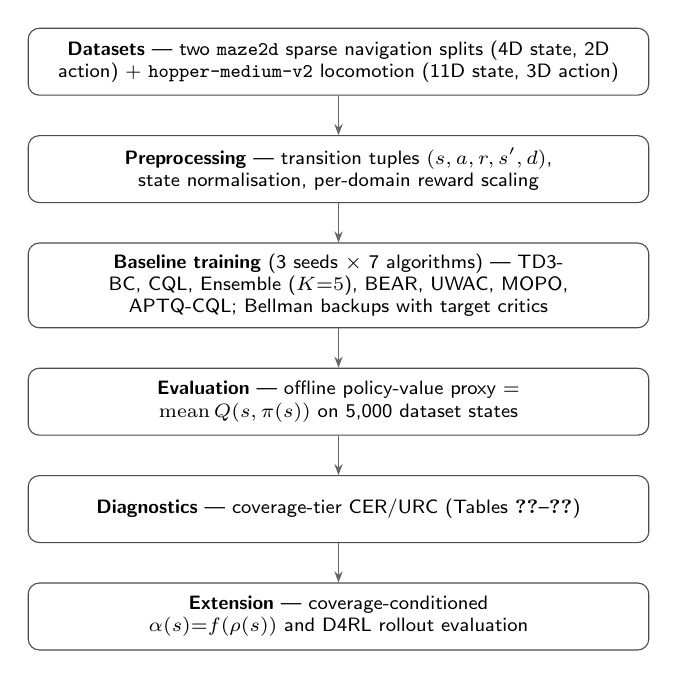
\begin{tikzpicture}[node distance=0.5cm]
  \node[pbox] (data)
    {\textbf{Datasets} --- two \texttt{maze2d} sparse navigation splits
     (4D state, 2D action) + \texttt{hopper-medium-v2} locomotion
     (11D state, 3D action)};
  \node[pbox,below=of data] (pre)
    {\textbf{Preprocessing} --- transition tuples $(s,a,r,s',d)$,
     state normalisation, per-domain reward scaling};
  \node[pbox,below=of pre] (train)
    {\textbf{Baseline training} (3 seeds $\times$ 7 algorithms) ---
     TD3-BC, CQL, Ensemble ($K{=}5$), BEAR, UWAC, MOPO, APTQ-CQL;
     Bellman backups with target critics};
  \node[pbox,below=of train] (eval)
    {\textbf{Evaluation} --- offline policy-value proxy
     $=\mathrm{mean}\,Q(s,\pi(s))$ on 5{,}000 dataset states};
  \node[pbox,below=of eval] (res)
    {\textbf{Diagnostics} --- coverage-tier CER/URC
     (Tables~\ref{tab:perf}--\ref{tab:diag})};
  \node[pbox,below=of res] (next)
    {\textbf{Extension} --- coverage-conditioned
     $\alpha(s){=}f(\rho(s))$ and D4RL rollout evaluation};
  \draw[arr] (data) -- (pre);
  \draw[arr] (pre)  -- (train);
  \draw[arr] (train)-- (eval);
  \draw[arr] (eval) -- (res);
  \draw[arr] (res)  -- (next);
\end{tikzpicture}
\caption{Empirical pipeline applied identically to all three datasets:
matched training, unified proxy evaluation, and coverage-tier diagnostics.}
\label{fig:pipeline}
\end{figure}

\section{Experimental Setup}
\label{sec:setup}

\subsection{Datasets}

We use three D4RL datasets~\cite{fu2020d4rl}.
\texttt{maze2d-medium-sparse-v1} and \texttt{maze2d-large-sparse-v1} contain
transitions from a waypoint-following controller in medium- and
large-complexity 2D mazes; the 4D state encodes position and velocity, the
2D action is continuous, coverage is dense along demonstrated paths and
near-zero in unvisited corridors, and rewards are sparse and
goal-conditioned. \texttt{hopper-medium-v2} is a single-leg locomotion task
with an 11D state, a 3D continuous action, and dense shaped rewards from a
medium-level policy. Together the three span the two coverage regimes that a
fixed $\alpha$ must reconcile: structured sparse navigation versus densely
covered continuous control.

\subsection{Algorithms and Validation Protocol}

All seven algorithms are trained under the matched protocol of
Table~\ref{tab:hparams} for three independent seeds
($\mathrm{seed}\in\{0,1,2\}$), with \texttt{torch}, \texttt{numpy}, and
Python random seeds set per run. The reported score for each run is the mean
of the final three evaluation points of the training curve; the table entry
is the mean $\pm$ standard deviation across the three seeds.

\begin{table}[t]
\centering
\caption{Shared hyperparameters (all algorithms, all datasets)}
\label{tab:hparams}
\setlength{\tabcolsep}{4pt}
\begin{tabular}{ll}
\toprule
\textbf{Parameter} & \textbf{Value} \\
\midrule
Network & 256--256 MLP actor/critic \\
Optimiser / lr & Adam, $3{\times}10^{-4}$ \\
Batch size & 256 \\
Discount $\gamma$ & 0.99 \\
Target smoothing $\tau$ & 0.005 \\
Training budget & $10 \times 200$ grad.\ steps / seed \\
Bellman target clip & $\pm 10$ \\
Reward scale & $1.0$ (maze) / $10^{-2}$ (hopper) \\
CQL $\alpha$ & 1.0 (fixed); APTQ adapts in $[0.5,5]$ \\
BC weight $\lambda$ & 0.1 \\
Ensemble size $K$ & 5 \\
Eval.\ states & 5{,}000 (first transitions) \\
Seeds & $\{0,1,2\}$ \\
\bottomrule
\end{tabular}
\end{table}

\subsection{Evaluation Metric}

All algorithms share a single offline evaluation protocol. At each
checkpoint the policy $\pi$ and critic(s) are frozen and the score is the
mean of $Q(s,\pi(s))$ over the first 5{,}000 transitions. This policy-value
proxy enables fair cross-algorithm comparison under identical budgets, but
it is \emph{not} a D4RL rollout or normalised return~\cite{fu2020d4rl}, and
its magnitude depends on the per-domain reward scale (hopper $Q$ values are
correspondingly larger than maze ones). Comparisons are therefore made
\emph{within} a dataset. Environment rollouts with official D4RL
normalisation are left to future work.

\subsection{Diagnostic Protocol}

Coverage tiers are computed via $k$NN density (Eq.~\ref{eq:coverage},
$k{=}10$) on a stratified subsample of $5{\times}10^{4}$ transitions per
dataset. $Q_{\mathrm{BC}}$ is a critic regressed onto per-transition Monte
Carlo returns $G_i$; $u(s,a)$ is the standard deviation across a five-member
ensemble trained on the same targets. CER and URC
(Eqs.~\ref{eq:cer}--\ref{eq:urc}) are reported per tier for CQL and
APTQ-CQL (seed~0 checkpoints).

\section{Results and Analysis}
\label{sec:results}

\begin{table*}[t]
\centering
\caption{Unified offline policy-value proxy across three datasets
(mean $\pm$ std over 3 seeds; higher is better, best per column in bold).
Scores are within-dataset critic means and are not comparable across
columns owing to differing reward scales.}
\label{tab:perf}
\setlength{\tabcolsep}{12pt}
\begin{tabular}{lccc}
\toprule
 & \multicolumn{2}{c}{\textbf{Navigation (maze2d, sparse)}} & \textbf{Locomotion (dense)} \\
\cmidrule(lr){2-3}\cmidrule(lr){4-4}
\textbf{Algorithm} & \texttt{medium-sparse-v1} & \texttt{large-sparse-v1} & \texttt{hopper-medium-v2} \\
\midrule
CQL~\cite{kumar2020conservative}      & $\mathbf{2.293 \pm 0.141}$ & $\mathbf{2.899 \pm 0.061}$ & $\mathbf{11.881 \pm 0.121}$ \\
APTQ-CQL~\cite{liu2023aptq}           & $1.333 \pm 0.143$ & $1.632 \pm 0.050$ & $8.919 \pm 0.163$ \\
UWAC~\cite{wu2021uncertainty}         & $0.144 \pm 0.016$ & $0.268 \pm 0.004$ & $0.530 \pm 0.116$ \\
Ensemble~\cite{an2021pbrl}            & $0.118 \pm 0.010$ & $0.222 \pm 0.010$ & $0.307 \pm 0.044$ \\
TD3-BC~\cite{fujimoto2021td3bc}       & $0.112 \pm 0.023$ & $0.202 \pm 0.030$ & $0.372 \pm 0.122$ \\
MOPO~\cite{yu2020mopo}                & $0.014 \pm 0.001$ & $0.024 \pm 0.004$ & $0.029 \pm 0.000$ \\
BEAR~\cite{kumar2019bear}             & $-0.001 \pm 0.054$ & $0.105 \pm 0.015$ & $0.328 \pm 1.434$ \\
\bottomrule
\end{tabular}
\end{table*}

\begin{figure*}[t]
\centering
\begin{subfigure}{0.32\textwidth}
  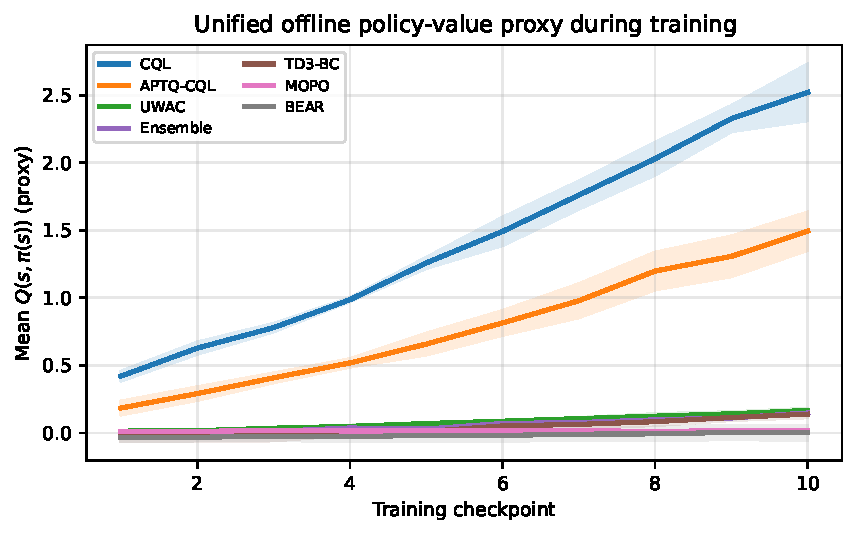
\includegraphics[width=\linewidth]{figures/training_curves.pdf}
  \caption{maze2d-medium-sparse}
\end{subfigure}\hfill
\begin{subfigure}{0.32\textwidth}
  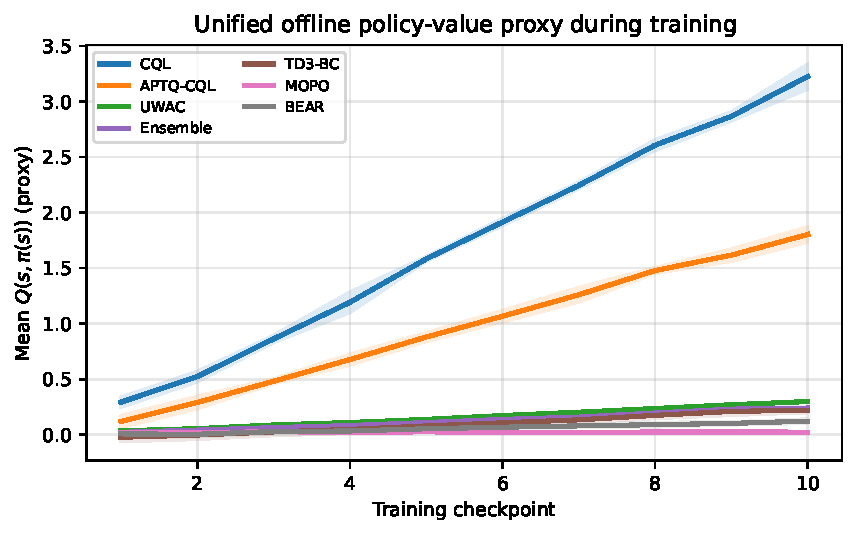
\includegraphics[width=\linewidth]{figures/large_training_curves.pdf}
  \caption{maze2d-large-sparse}
\end{subfigure}\hfill
\begin{subfigure}{0.32\textwidth}
  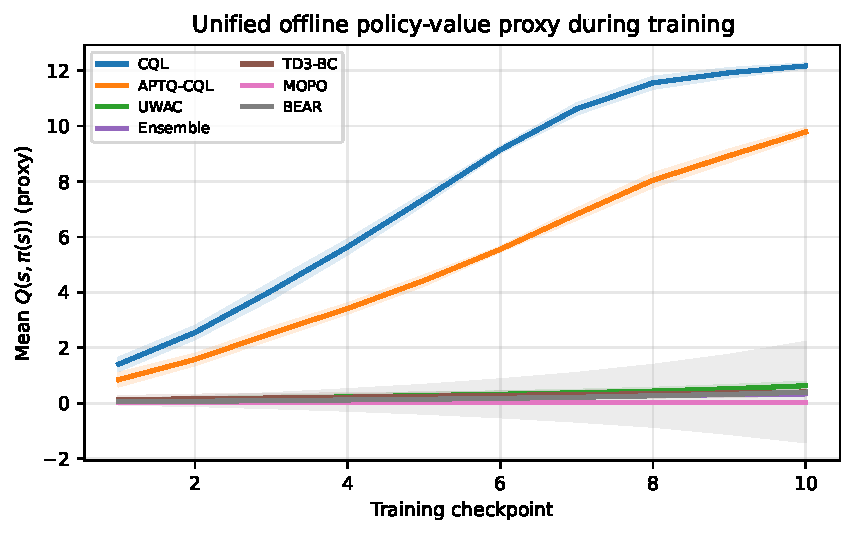
\includegraphics[width=\linewidth]{figures/hopper_training_curves.pdf}
  \caption{hopper-medium-v2}
\end{subfigure}
\caption{Unified offline proxy score during training (mean $\pm$ std over
three seeds). CQL and APTQ-CQL separate early from the remaining baselines on
every dataset; note the larger $y$-scale on hopper from its dense rewards.}
\label{fig:curves}
\end{figure*}

Table~\ref{tab:perf} summarises proxy scores. The ranking is
\emph{remarkably stable across all three datasets}:
\textbf{CQL}~\cite{kumar2020conservative} ranks highest at fixed
$\alpha{=}1.0$, \textbf{APTQ-CQL}~\cite{liu2023aptq} is a clear second, and
the support-/uncertainty-based baselines (UWAC, Ensemble, TD3-BC) cluster an
order of magnitude lower, with MOPO and BEAR last. The CQL/APTQ-CQL gap
persists from the sparse mazes to dense hopper, indicating that the
advantage of explicit value pessimism under this matched budget is not an
artefact of a single coverage regime. Because scores are raw critic means
rather than normalised returns, each column is a within-study ranking only.
Figure~\ref{fig:curves} shows the corresponding learning dynamics: on all
three datasets CQL and APTQ-CQL grow steadily while the other methods remain
flat near zero (BEAR additionally exhibits large inter-seed variance on
hopper).

\section{Coverage-Tier Diagnostics}
\label{sec:diagnostics}

\begin{table*}[t]
\centering
\caption{Coverage-tier diagnostics ($5{\times}10^{4}$-transition subsample,
$k{=}10$). CER is reported per method; URC measures uncertainty vs.\ return
and is method-independent within a dataset (reported once).}
\label{tab:diag}
\setlength{\tabcolsep}{7pt}
\begin{tabular}{ll ccc ccc}
\toprule
& & \multicolumn{3}{c}{\textbf{CER}} & \multicolumn{3}{c}{\textbf{URC}} \\
\cmidrule(lr){3-5}\cmidrule(lr){6-8}
\textbf{Dataset} & \textbf{Method} & High & Med & Low & High & Med & Low \\
\midrule
\multirow{2}{*}{\texttt{maze2d-medium-sparse}}
  & CQL      & $-14.47$ & $-16.58$ & $-17.56$ & \multirow{2}{*}{$+0.54$} & \multirow{2}{*}{$+0.52$} & \multirow{2}{*}{$+0.48$} \\
  & APTQ-CQL & $-3.11$  & $-3.94$  & $-5.03$  & & & \\
\midrule
\multirow{2}{*}{\texttt{maze2d-large-sparse}}
  & CQL      & $-33.74$ & $-31.59$ & $-31.96$ & \multirow{2}{*}{$+0.25$} & \multirow{2}{*}{$+0.36$} & \multirow{2}{*}{$+0.51$} \\
  & APTQ-CQL & $-16.49$ & $-15.06$ & $-14.78$ & & & \\
\midrule
\multirow{2}{*}{\texttt{hopper-medium-v2}}
  & CQL      & $-134.9$ & $-138.2$ & $-142.8$ & \multirow{2}{*}{$-0.20$} & \multirow{2}{*}{$-0.21$} & \multirow{2}{*}{$-0.28$} \\
  & APTQ-CQL & $-92.3$  & $-114.6$ & $-120.5$ & & & \\
\bottomrule
\end{tabular}
\end{table*}

\begin{figure*}[t]
\centering
\begin{subfigure}{0.32\textwidth}
  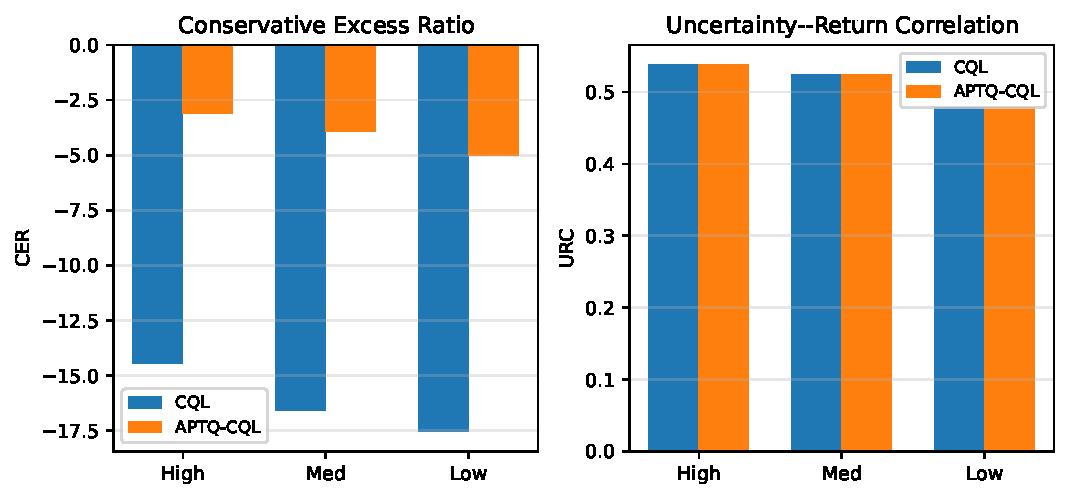
\includegraphics[width=\linewidth]{figures/cer_urc.pdf}
  \caption{maze2d-medium-sparse}
\end{subfigure}\hfill
\begin{subfigure}{0.32\textwidth}
  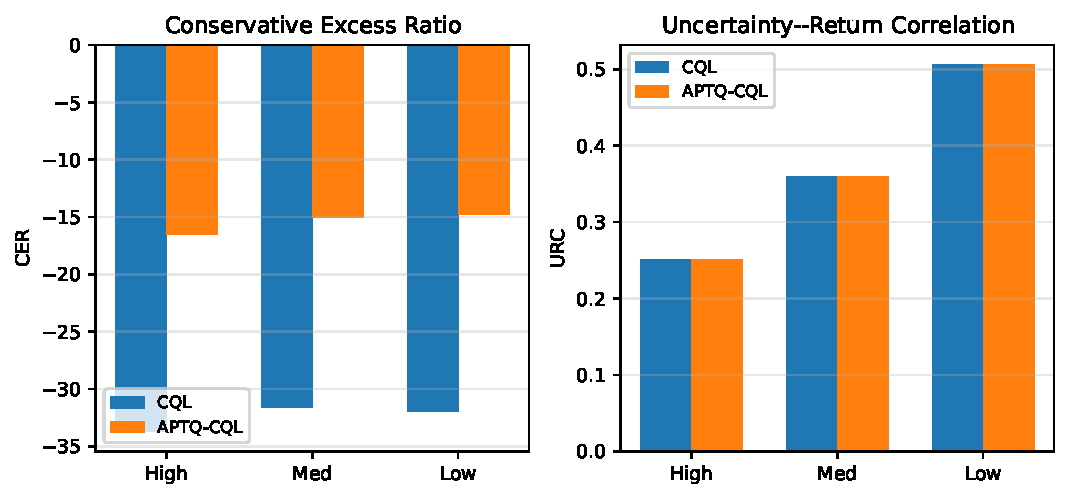
\includegraphics[width=\linewidth]{figures/large_cer_urc.pdf}
  \caption{maze2d-large-sparse}
\end{subfigure}\hfill
\begin{subfigure}{0.32\textwidth}
  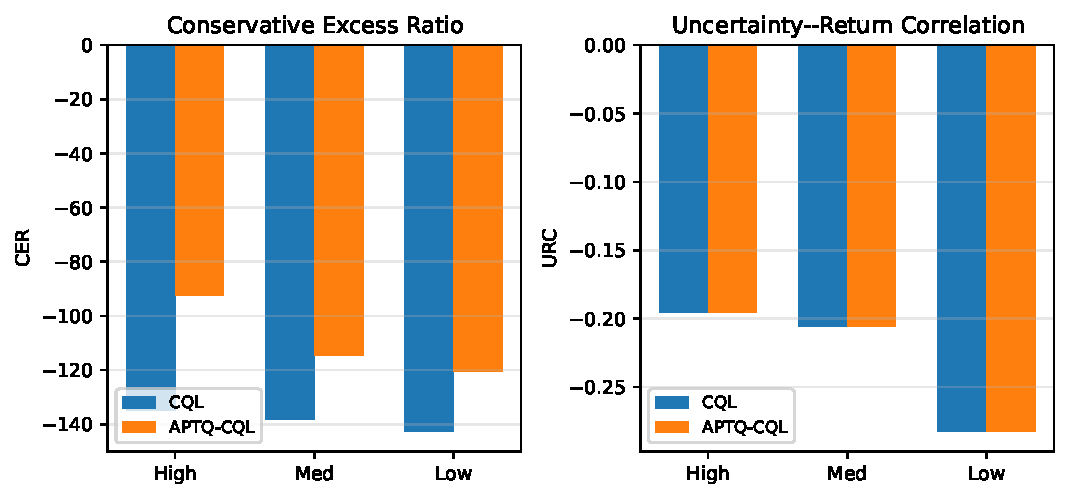
\includegraphics[width=\linewidth]{figures/hopper_cer_urc.pdf}
  \caption{hopper-medium-v2}
\end{subfigure}
\caption{Coverage-tier CER (left of each panel) and URC (right) for CQL and
APTQ-CQL. CER is negative in every tier and dataset (CQL more so than
APTQ-CQL). URC is positive on both sparse mazes but negative on hopper---the
sign flip is the central cross-domain finding.}
\label{fig:diag}
\end{figure*}

\begin{figure*}[t]
\centering
\begin{subfigure}{0.30\textwidth}
  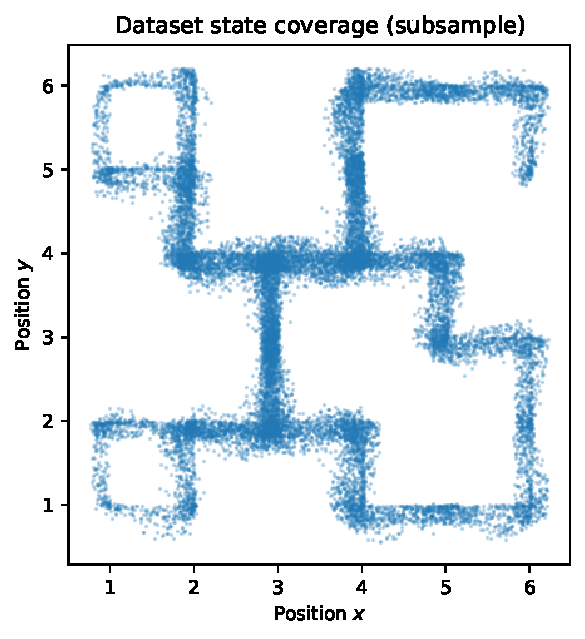
\includegraphics[width=\linewidth]{figures/coverage_map.pdf}
  \caption{maze2d-medium-sparse ($x,y$)}
\end{subfigure}\hfill
\begin{subfigure}{0.30\textwidth}
  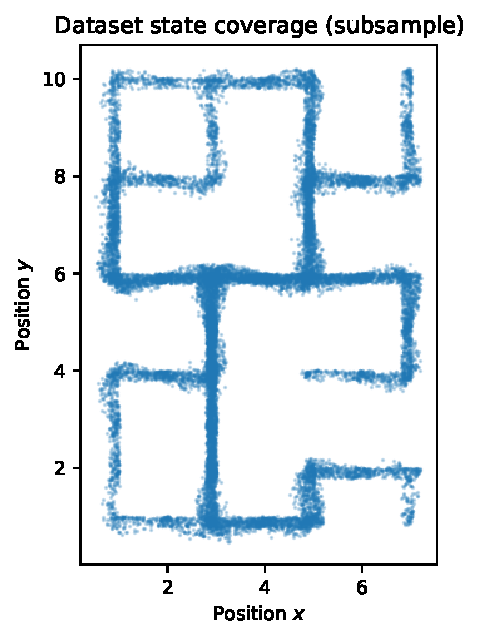
\includegraphics[width=\linewidth]{figures/large_coverage_map.pdf}
  \caption{maze2d-large-sparse ($x,y$)}
\end{subfigure}\hfill
\begin{subfigure}{0.30\textwidth}
  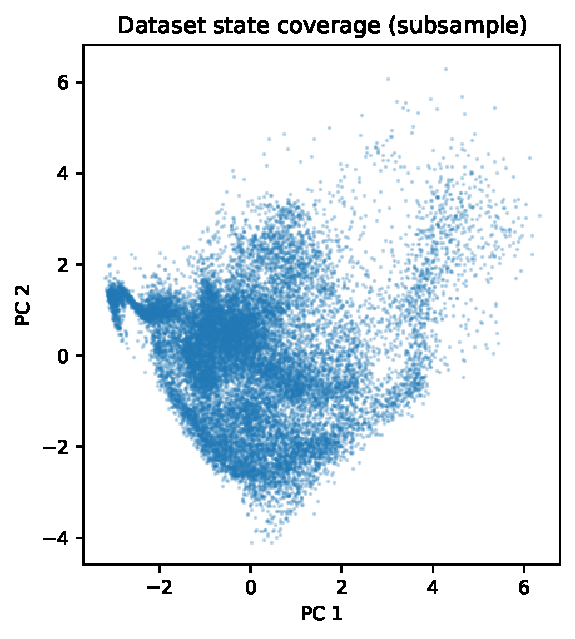
\includegraphics[width=\linewidth]{figures/hopper_coverage_map.pdf}
  \caption{hopper-medium-v2 (PC1, PC2)}
\end{subfigure}
\caption{State coverage (20k-point subsample). The mazes show
path-concentrated support with empty corridors; hopper (top-2 principal
components of the standardised state) shows a dense core that tapers into
sparse high-velocity excursions.}
\label{fig:coverage}
\end{figure*}

Table~\ref{tab:diag} and Figure~\ref{fig:diag} test the spatial
miscalibration hypothesis directly. Three patterns are consistent across all
datasets. First, \textbf{$\mathrm{CER}{<}0$ in every tier} for both methods,
i.e.\ $Q_{\mathrm{algo}}>Q_{\mathrm{BC}}$: under the matched short budget,
fixed-$\alpha$ CQL is \emph{optimistic} relative to the Monte Carlo value
baseline, not over-conservative. Second, \textbf{APTQ-CQL consistently
reduces this excess}---most strongly in well-covered tiers (e.g.\ the
high-tier gap narrows from $-14.47$ to $-3.11$ on medium-maze and from
$-134.9$ to $-92.3$ on hopper)---indicating that global penalty adaptation
helps most precisely where data are abundant. Third, on the sparse mazes the
optimism tends to grow toward low-coverage regions ($|\mathrm{CER}|$
largest in the Low tier), consistent with insufficient pessimism where data
are scarce; on dense hopper the same low-tier worsening appears for both
methods.

The decisive cross-domain result is the \textbf{sign of URC}. On both sparse
mazes, $\mathrm{URC}{>}0$ in every tier ($+0.25$ to $+0.54$): higher
ensemble disagreement co-occurs with \emph{higher} Monte Carlo
return---likely because rare goal-reaching segments are locally
heterogeneous---so $u(s,a)$ is an unreliable, even misleading, calibration
signal without tier conditioning. On \texttt{hopper-medium-v2}, by contrast,
$\mathrm{URC}{<}0$ in every tier ($-0.20$ to $-0.28$) and becomes most
negative in the Low tier: here uncertainty behaves as theory expects,
anticorrelating with return. Ensemble disagreement is therefore a usable
pessimism signal in the densely covered locomotion domain but not in the
path-concentrated mazes. Figure~\ref{fig:coverage} makes the underlying
support geometry concrete: the mazes are dominated by thin demonstrated
corridors surrounded by empty space, whereas hopper fills a dense core.

\section{Discussion}
\label{sec:discussion}

\subsection{What the results establish}

The stable ranking (Table~\ref{tab:perf}) separates explicit CQL-style
critics from lighter baselines across both domains, but the tier diagnostics
(Table~\ref{tab:diag}) refine the miscalibration story: a fixed global
$\alpha$ does not over-penalise well-covered regions---it remains optimistic
relative to $Q_{\mathrm{BC}}$ everywhere, with the largest optimism where
coverage is lowest. This is more consistent with \emph{under}-penalisation of
OOD value than with over-penalisation along paths, and it motivates
spatially conditioned conservatism rather than a uniform scalar reduction of
$\alpha$. The URC sign flip further shows that the natural ingredient for
such conditioning---ensemble uncertainty---is informative in dense
locomotion but unreliable in sparse navigation, so a coverage-conditioned
scheme should lean on density $\rho(s)$ directly rather than on $u(s,a)$
alone in the sparse regime.

\subsection{From global to spatial adaptation}

APTQ's adaptation is \emph{temporal and global}: $\alpha_t$ in
Eq.~\eqref{eq:aptq} is shared by every transition at step $t$. Its
consistent second place and uniform reduction of CER show that adaptive
pessimism is competitive with fixed $\alpha$, but it cannot exploit the
spatial structure that Table~\ref{tab:diag} exposes. The natural next
experiment replaces the scalar $\alpha$ with a per-sample penalty
$\alpha(s)=f(\rho(s))$ keyed to the coverage density of
Eq.~\eqref{eq:coverage}, then re-evaluates CER/URC and D4RL rollout return.

\subsection{Lower-tier baselines}

BEAR, TD3-BC, Ensemble, and UWAC cluster well below the CQL family on all
three datasets, and MOPO is lowest. Under the simplified budget used here,
support constraints, uncertainty reweighting, and short model rollouts do
not by themselves yield critics whose policy-implied values match CQL-style
methods---an observation that holds in both the sparse and dense regimes.

\subsection{Limitations}

\textbf{Implementation scope.} Results use compact educational
reimplementations with a short training budget, not official author
codebases or tuned hyperparameters; absolute magnitudes are not D4RL scores.
\textbf{Evaluation scope.} Proxy $Q$ scores are not normalised returns, are
not comparable across datasets, and three seeds limit statistical power.
\textbf{Diagnostics scope.} CER/URC rely on ensemble uncertainty trained on
Monte Carlo targets and a single checkpoint per method; they indicate
calibration patterns but do not prove a causal benefit of spatial
$\alpha(s)$. \textbf{Next steps.} (i)~D4RL rollouts with MuJoCo; (ii)~more
locomotion levels (medium-replay, expert) and additional maze sizes;
(iii)~coverage-conditioned $\alpha(s){=}f(\rho(s))$ with tier-aware
evaluation; (iv)~implicit-Q and AWAC baselines.

\section{Conclusion}
\label{sec:conclusion}

This paper compares seven offline RL baselines across three D4RL datasets
spanning sparse navigation and dense locomotion, under matched training and a
unified offline evaluation protocol, augmented with coverage-tier CER/URC
diagnostics. The proxy ranking is stable across all three datasets:
fixed-$\alpha$ CQL is highest and APTQ-CQL second. Yet in every tier and
dataset both methods are optimistic relative to a Monte Carlo value
baseline ($\mathrm{CER}{<}0$), with the largest optimism where coverage is
lowest, and APTQ-CQL attenuates this excess most on well-covered states.
Finally, the uncertainty--return correlation flips sign between domains---
positive on the sparse mazes, negative on hopper---showing that ensemble
disagreement is a dependable calibration signal only where coverage is
dense. Together these results argue for coverage-aware pessimism
$\alpha(s){=}f(\rho(s))$, evaluated with environment-level D4RL returns, as
the next step.

\begin{thebibliography}{10}

\bibitem{levine2020offline}
S.~Levine, A.~Kumar, G.~Tucker, and J.~Fu,
``Offline reinforcement learning: Tutorial, review, and perspectives on open
problems,'' \textit{arXiv:2005.01643}, 2020.

\bibitem{fujimoto2019bcq}
S.~Fujimoto, D.~Meger, and D.~Precup,
``Off-policy deep reinforcement learning without exploration,''
in \textit{Proc.\ ICML}, pp.~2052--2062, 2019.

\bibitem{kumar2020conservative}
A.~Kumar, A.~Zhou, G.~Tucker, and S.~Levine,
``Conservative Q-learning for offline reinforcement learning,''
in \textit{Proc.\ NeurIPS}, vol.~33, pp.~1179--1191, 2020.

\bibitem{an2021pbrl}
G.~An, S.~Moon, J.-H. Kim, and H.~O. Song,
``Uncertainty-based offline reinforcement learning with diversified
Q-ensemble,''
in \textit{Proc.\ NeurIPS}, vol.~34, pp.~7436--7447, 2021.

\bibitem{wu2021uncertainty}
Y.~Wu, S.~Tucker, and O.~Nachum,
``Uncertainty weighted actor-critic for offline reinforcement learning,''
\textit{arXiv:2105.08140}, 2021.

\bibitem{liu2023aptq}
Y.~Liu, B.~Zhang, J.~Li, and Z.~Zhang,
``APTQ: Adaptive pessimism-based offline reinforcement learning with
Q-value target,''
\textit{arXiv:2307.13702}, 2023.

\bibitem{fu2020d4rl}
J.~Fu, A.~Kumar, O.~Nachum, G.~Tucker, and S.~Levine,
``D4RL: Datasets for deep data-driven reinforcement learning,''
\textit{arXiv:2004.07219}, 2020.

\bibitem{fujimoto2021td3bc}
S.~Fujimoto and S.~S. Gu,
``A minimalist approach to offline reinforcement learning,''
in \textit{Proc.\ NeurIPS}, vol.~34, pp.~20132--20145, 2021.

\bibitem{kumar2019bear}
A.~Kumar, J.~Fu, M.~Soh, G.~Tucker, and S.~Levine,
``Stabilising off-policy Q-learning via bootstrapping error reduction,''
in \textit{Proc.\ NeurIPS}, vol.~32, 2019.

\bibitem{yu2020mopo}
T.~Yu \textit{et al.},
``MOPO: Model-based offline policy optimisation,''
in \textit{Proc.\ NeurIPS}, vol.~33, pp.~14129--14142, 2020.

\end{thebibliography}

\end{document}
